% !TEX root = ../thesis.tex
% [H] means put the figure HERE, directly when you input this code.
% Remove this to let LaTeX place the figure where it decides is best
\begin{figure}
	\centering

	% We set the width of the figure based on the width of one line 
	% of text on the page. The value can be tuned to any value in 
	% [0.0, 1.0] to scale the image while maintaining its aspect ratio.
	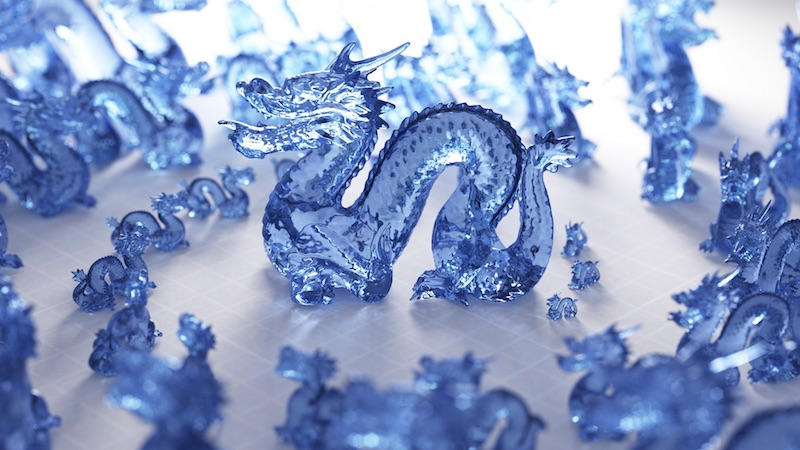
\includegraphics[width=1.0\textwidth]{dragon.jpg}
	
	% Caption is defined with a short and long version. The short 
	% version is shown in the List of Figures section, and the long 
	% version is used directly with the figure. 		
	\caption[Short caption.]{Long caption and citation \cite{whittle15_dragons}.
	
	% Figure labels should be defined at the end of the caption to
	% ensure proper numbering.
	\label{fig:dragon}
	}
\end{figure}